%Preamble to set up the document
\documentclass[12pt]{report}
\usepackage[margin=1.0in]{geometry}
\usepackage{graphicx}
\usepackage{amsmath}
\usepackage{amssymb}
\author{Fajans Lab and \& Friends}
\title{Code Documentation}

\begin{document}
\maketitle

\chapter*{Preface}
This file is intended to act as a manual for all of the code used for the Lorentz Invariance investigations.  It is a work in progress and you should feel free to edit it.  The version tracking is performed by git and you may download this software from Github.  The Github repository is private, so send Zak an email at uphgreat@gmail.com containing your Github username if you would like access.

\tableofcontents



%Here we start the real documentation
\chapter{Analysis Class}
The analysis class is designed to allow the user to perform all the high level tasks necessary for the analysis, so if you want to use the code but don't want to read this whole lengthy manual, just read through this chapter.  Each analysis instance is designed to work with one generate\_event\_times() function (since we expect to pick one and stick with it in the end).  This class inherits from Matlab's handle class, so references to it act like pointers.

\section{Set-up/Initialization}
The first step to create an Analysis instance is to decide which generate\_event\_times() function you would like to use.  Several versions are included in the code, each one residing in its own subdirectory of SimulationData/DataSets/.  The names of the subdirectories are used to identify the different versions of that function.  You may add your own version in its own subdirectory there if you desire.  Make sure no functions with the name generate\_event\_times() are available in your path; that will disrupt the inner workings of the Analysis class and cause it to throw an error.  The Analysis class will automatically add the appropriate directories to the path variable when an instance is created.

Now you are ready to initialize an instance of this class.  To do this, change to the directory\footnote{The paths used internally are relative to SimulationData/code/Classes, so make sure this is your working directory; do not just add it to your path} SimulationData/code/Classes.  Now call the constructor with the name of the generate\_event\_times.m folder as the only argument (just the name of the folder, not the path to it) as shown below.  This will automatically create the subdirectories necessary and will warn you if there are issues.

Since the whole analysis process can take a long time, a lot of results are saved to the hard drive so that future instances of the Analysis class can have the results without having to recalculate them.  Therefore, if you've already run an analysis, you can get a lot of the data back just be creating another Analysis instance for the same folder and using its load functions (which are automatically called when you create the instance for the important data).

\begin{verbatim}
>> four_month=Analysis('FourMonth')

four_month = 

  Analysis with properties:

       GENERATOR_NAME: 'FourMonth'
    signal_group_list: {1x6 cell}
            n_workers: []
        data_set_root: '../../DataSets/FourMonth'

\end{verbatim}

\section{Running the Analysis}
Running the analysis is a two-step process.  First, tell the the analysis instance what kind of signals you would like it to simulate.  The easiest way to do this is to use Analysis.simple\_add\_sine().  This function takes at least one argument: the amplitude of the fractional charge variation, which should be on the order of ~$\sim 1 \times 10^{-8}$.  You may optionally also specify 'period', 'phase', or 'n\_sets'.

You can also add your own function for picking charge values as a function of time, velocity, etc.  Be careful when doing this though, because Matlab stores all workspace variables when you create a function handle, which can include all the tracer data if you have an Analysis instance open.  This causes issues when the code saves the function handle to the hard drive because it will include a copy of all the tracer data.  To add your own function, first add the desired signal\_group instances to the analysis instance by using the analysis.add\_signal\_group() method.  The method requires a function handle as an input, and you can optionally also pass it a string, which sets the signal\_group's signal\_name attribute, and/or a number, which tells it how many data sets to generate.  The function handle should be a function which takes a data\_set and modifies it to add a signal to the raw data.  Two such functions are included: signal\_null() and signal\_sine().  By default, two signal\_groups are added when you create an analysis instance, one for each of these.  You may also want to add other signal\_sine groups with different amplitudes, frequencies, or phases.  You may remove a signal\_group by using the analysis.delete\_signal\_group() method, which takes a signal\_name, or by using analysis.pop\_signal\_group() which deletes the most recently added signal\_group.

Once the desired signal groups are added, the data for all the various signal groups can be generated simply by calling analysis.run().  This will create all the data\_sets, use Andy's Charman IV algorithm on them, store the results, and generate a nice histogram showing the results of the first and last signal\_groups.

After running the analysis, more signal\_groups can be added or deleted, then analysis.run() can be called again to generate the data and the histogram.  If all the desired data has been generated, you may call analysis.generate\_Charman\_histograms() directly and specify which signal\_groups to plot and how many bins to use.

\begin{verbatim}
>> four_month.add_signal_group(@(data_set)signal_sine(data_set,0.01,'day',pi/8),'delayed daily sine',100)
>> four_month.run()
Generating data for signal group null...
Done. Took 4.56 seconds

Generating data for signal group daily sine...
Done. Took 5.45 seconds

Generating data for signal group delayed daily sine...
Done. Took 5.00 seconds


Generating Charman histograms...
Finished generating Charman histograms
Generating Charman histograms took 0.22 seconds


>> four_month.generate_Charman_histograms({'null','daily sine','delayed daily sine'},25)
Generating Charman histograms...
Done.  Took 0.22 seconds
\end{verbatim}

\section{Analysis.add\_signal\_group()}
This method creates a signal\_group and adds it to analysis.signal\_group\_list.  You must give it a function handle that accepts a data\_set as an input, then returns an array of charges.  You may create your own signal functions, or you may use the provided ones, which are discussed in Chapter \ref{chap:SignalFunctions}.

You may also specify a signal\_name, which you will use to identify the signal\_group when you interact with it (plot its data, delete it, etc.).  If you do not specify a name, one will be generated automatically using the Analysis.func\_to\_signal\_name() method.  Furthermore, you may specify a number of data\_sets to generate for that signal\_group.  If you do not provide a value, it will allow the Signal\_Group constructor to choose the default value (which is currently set to 100).

If you choose to use the signal\_sine function for a signal\_group (and you most likely will), you will have to provide some arguments in the function handle for the amplitude, period, and phase.  This is because the function handle given to Analysis.add\_signal\_group() must take only one argument: the data\_set.  See the examples of valid uses below.

Another point worth noting is that the code is smart enough to stop you from adding two signal\_groups with the same signal\_names, and it is smart enough to stop you from adding the same function handle twice.  If you attempt to do this, it will not create a new signal\_group and it will display a warning.

To remove a signal\_group from analysis.signal\_group\_list (this will also delete all its data from the hard drive), you may call Analysis.delete\_signal\_group() with the signal\_name of the signal\_group as the only argument.  Another alternative is to use Analysis.pop\_signal\_group(), which automatically deletes the signal\_group at the end of analysis.signal\_group\_list (which is the most recently added one).

\begin{verbatim}
>> four_month.add_signal_group(@(data_set)null(data_set),'null')
Warning: The given function name null is already in self.signal_group_list 
> In Analysis>Analysis.add_signal_group at 202 
>> four_month.add_signal_group(@(data_set)signal_sine(data_set,0.02,'day',0));
>> four_month.add_signal_group(@(data_set) ...
signal_sine(data_set,0.02,'day',pi/8),'delayed sine',500);
\end{verbatim}

\section{Analysis.generate\_Charman\_histograms()}
This method produces a histogram that appears as a docked figure.  You may call it with no arguments, in which case it will by default plot the first (which is usually the null signal\_group) and the most recently added signal\_group with 30 bins.  Passing it a number will specify the number of bins.  Passing it a cell array with signal\_names will make it plot the data from the specified signal\_groups.

The most bins you can reasonably have with the data from LargeSimData is ${\sim}$30, but AllSimData looks good up to at least ${\sim}$100 bins.  Currently, this function does not save the figures, but they can be saved with the savefig() command.

\begin{verbatim}
>> four_month.generate_Charman_histograms({'null','daily sine','delayed daily sine'},25)
Generating Charman histograms...
Done.  Took 0.31 seconds
\end{verbatim}





\chapter{Signal\_Group Class}
You should not need to interact directly with this class very often.  Instances of this class are stored in the Analysis.signal\_group\_list property.  The only time I expect that a person would want to interact with it directly would be if they wanted to change the number of data\_sets that are generated for that signal\_group.  This can be done with the Signal\_Group.set\_n\_sets() method, which takes one argument: n\_sets.  If n\_sets is 0, the signal\_group will automatically set it to its default value (right now that is 100).  Note that if n\_sets increases, the new data\_sets will not be generated immediately.  To generate additional data\_sets, call analysis.run()

\begin{verbatim}
>> four_month.signal_group_list{1}.set_n_sets(1000)
>> four_month.run()
Generating data for signal group null...
Done. Took 47.21 seconds
blah blah blah....
\end{verbatim}





\chapter{Data\_Set Classes}
\label{chap:DataSet}
This chapter discusses Data\_Sets, Raw\_Data\_Sets and Calc\_Data\_Sets.  The overall structure is that each instance of the Data\_Set class manages an instance of the Raw\_Data\_Set class and an instance of the Calc\_Data\_Set class.  Each raw\_data\_set contains the times and $z$-positions of the events, and each calc\_data\_set contains the calculated data (for now this is just the cmb velocity).  The Data\_Set class exists because the data in the Raw\_Data\_Set and Calc\_Data\_Set instances takes up a lot of memory, so the Data\_Set class keeps them organized and saves/loads them to/from the hard drive to save RAM.

\section{Data\_Set Class}
An instance of the Data\_Set class can create a Raw\_Data\_Set, then save it to the hard drive and erase it from RAM to save space.  It can also take the information in a Raw\_Data\_Set and use it to create a Calc\_Data\_Set instance, which it can then save to the hard drive and unload from RAM.  Instances of the Calc\_Data\_Set can also load their corresponding Raw\_Data\_Set and Calc\_Data\_Set instances from the hard drive to access their data later.

Initializing a Data\_Set takes a lot of arguments, so the simplest way to get your hands on one is to create an Analysis instance then use the Analysis.get\_one\_data\_set() method, which takes no arguments and returns one Data\_Set instance.  Once you have a Data\_Set, its Raw\_Data\_Set can be created by Data\_Set.create\_raw\_data\_set(), which takes one array  and one constant as arguments.  The array should have two columns: the first containing date times and the second containing $z$-positions.  The constant specifies how many of the events are quip left (the first n\_left rows of the array are assumed to be quip left).  This can then be saved to the hard drive by calling Data\_Set.save\_raw\_data\_set().  Once the Raw\_Data\_Set is saved, it can be erased from memory by calling Data\_Set.unload\_raw\_data\_set() and then loaded again using Data\_Set.load\_raw\_data\_set().  Whenever the Raw\_Data\_Set is not loaded, Data\_Set.raw\_data\_set is set to be an empty array, so you can check whether or not the Raw\_Data\_Set is loaded by calling isempty(Data\_Set.raw\_data\_set).

The methods for the Calc\_Data\_Set are very similar, just change "raw" to "calc" in the method names.  The one notable difference is that Data\_Set.create\_calc\_data\_set(), which is used to initialize the Calc\_Data\_Set, takes no arguments but can only be called after a Raw\_Data\_Set instance has been created.

\section{Raw\_Data\_Set Class}
This class stores the date times, charges, and $z$-positions for one data set.  Each of these is separated into two arrays, one for quip left data and one for quip right data.  A Raw\_Data\_Set instance can be accessed from a Data\_Set instance as data\_set.raw\_data\_set.

Iterating over quip left vs. quip right data can be annoying, so to make this simpler, the class includes two methods: get\_data(direction\_index) and get\_date\_times(direction\_index).  For each of these, a direction\_index of 1 returns quip left data and direction\_index 2 returns quip right data.

\section{Calc\_Data\_Set Class}
This class stores the data that can be calculated for each event from the data in the Raw\_Data\_Set instance.  It was designed to store CMB velocities, moon positions, and sun positions, each in separate arrays for the quip left and quip right data.  Currently only CMB velocities are stored.  For easier access, this information can be retrieved from methods that take direction\_index as an argument (again 1 for left or 2 for right).  These methods are get\_velocity(), get\_moon\_position(), and get\_sun\_position(), although only get\_velocity() is implemented at the moment.





\chapter{Position\_Generator Class}
Need to write this.





\chapter{Random\_Generator Class}
Need to write this.





\chapter{Functions in SimulationData/Code/SignalFunctions}
\label{chap:SignalFunctions}
These functions are used to add signals to the raw data in data\_set instances.  Their names begin with "signal\_" and they can be used to create Signal\_Group instances in an Analysis instance.  Each takes a data\_set instance as an argument and does not return anything (the data\_sets are modified in place).  If you code your own signal function, I recommend basing it off of signal\_sine, which is described below.

\section{signal\_null.m}
This function does not touch the data in the data\_set instance.  It is by default the first signal\_group in an Analysis instance's signal\_group\_list under the signal\_name 'null'.  A signal\_group that uses this signal function can be added to an Analysis instance as demonstrated in the following example.  Note that the signal\_group will not be created if a signal\_group with the given name or function handle is already in analysis.signal\_group\_list, and the 'null' signal\_group is already included by default.

\begin{verbatim}
>> four_month.add_signal_group(@(data_set)signal_null(data_set),'null')
Warning: The given function name null is already in self.signal_group_list 
> In Analysis>Analysis.add_signal_group at 202 
\end{verbatim}

\section{signal\_sine.m}
This function takes four arguments.  The first is the data\_set, and the rest are the amplitude (in meters), period (in sidereal days), and phase (in radians).  However, the signal function of a Signal\_Group instance must take only one argument: the data\_set.  Therefore, to add a signal\_group to an Analysis instance with this signal function, the given function handle must supply the rest of the arguments, as demonstrated in the example below.

\begin{verbatim}
>> four_month.add_signal_group(@(data_set) ...
signal_sine(data_set,0.05,'day',pi/8),'delayed sine');
\end{verbatim}





\chapter{Functions in SimulationData/Code/OtherFunctions/}
The SimulationData/ directory contains a mixture of data files separated into different folders.  Because a lot of simulation data was generated\footnote{${\sim}$400MB of time and position data was output by the simulations, which in turn is saved in many different ways, thereby increasing disk usage significantly.}, only small portions of each form of data are included in the Dropbox and Git repository.  If you need larger portions of the data, contact Zak at uphgreat@gmail.com.

\section{load/save\_mat.m}
These functions allow arbitrary Matlab objects to be saved and loaded.  The function save\_mat takes a file\_name (which can include a path) and an object and saves the object with the given file\_name.  The load\_mat function simply takes a file\_name as an argument and returns the saved object.

\begin{verbatim}
>> some_array=rand(3)

some_array =

    0.8147    0.9134    0.2785
    0.9058    0.6324    0.5469
    0.1270    0.0975    0.9575

>> save_mat('some_file_name',some_array);
>> clear some_array
>> some_array=load_mat('some_file_name');
>> some_array

some_array =

    0.8147    0.9134    0.2785
    0.9058    0.6324    0.5469
    0.1270    0.0975    0.9575
\end{verbatim}

\section{filter\_table.m}
This function takes a table and unlimited filter pairs as arguments and returns a table in which some rows have been filtered out.  The easiest way to understand it's behavior is through example.  If you would like to only look at the rows in Charman\_table where the quip is to the left and the data\_set\_index is 1, call the function as shown below.  This function is used to take a large data table and pick out only the rows that you want.

\begin{verbatim}
>> Charman_table=four_month.signal_group_list{1}.Charman_table;
>> Charman_table(1:4,:)

ans = 

    data_set_index    direction            A_1             abs_A_1 
    ______________    _________    ___________________    _________

    1                 left              NaN+0i                  NaN
    1                 right        0.002504-0.0028301i    0.0037788
    1                 averaged     0.002504-0.0028301i    0.0037788
    2                 left              NaN+0i                  NaN

>> filtered_table=filter_table(Charman_table,'direction','right','data_set_index',5)

filtered_table = 

    data_set_index    direction            A_1              abs_A_1 
    ______________    _________    ____________________    _________

    5                 right        0.0010866+0.0018011i    0.0021035
\end{verbatim}





\chapter{Functions in SimulationData/Code/ParameterFunctions}
These functions take Data\_Set instances and a direction as an argument and return an array giving the value of a parameter of interest at the event times of either the quip left or quip right data points.  The argument direction is either 1 for left, or 2 for right; any other value causes an error.  The names of each of these functions begins with "param\_" to indicate their purpose.  The first function of this type is param\_speed() which returns the CMB speed of the Earth.  Other similar function will be added in the future, such as the boost $\gamma$, angle between the trap and its CMB velocity, or parameters regarding the moon or sun position.







\chapter{Functions in SimulationData/Code/Mex/}
\label{chap:Mex}
This chapter covers the Mex functions in Simulation data that are used to interface with the Aephem library.  It documents both how to compile the functions and how they are used by their corresponding Matlab wrappers.

\section{Set-Up}
After some code edits, the set up process has been simplified.  If your machine is able to compile Mex files, all that needs to be done is to compile Aephem and put it in the correct directory.  The code should be stored with the same directory structure as that of the Dropbox folder.  After downloading the tarball for Aephem (I use version 2.0.0-Canopus, which is the latest version as of this writing), the tarball should be extracted into the aephem-2.0.0 directory.  The directory name does not have any colons or spaces in it because this seems to cause trouble for the Mex compiler.  Run 'make' to build the code.  If you've already built the code, you can just move the directory containing the code to the appropriate place (in the same directory as SimulationData/) and rename it to "aephem-2.0.0".  Or if you prefer not to have two copies of the software floating around, you might be able to get away with creating symbolic links.

If you have not used Mex on your machine before, it may need to be set up.  I ran 'mex -setup' before I tried compiling anything, but this may not have been necessary.  If you cannot build, refer to Matlab's documention for further instructions on getting Mex working.

\section{moon/sun\_position.c}
These functions are intended to be compiled with Mex.  After being successfully compiled, they take an array of Unix times and return three arrays giving the positions of the moon or sun: altitude angle (in degrees), azimuth angle (in degrees), and distance (in AU) in that order.

Because the input times are in Unix time, and because the libaephem library must be loaded before this function can run, wrapper functions datenum\_to\_moon\_position() and datenum\_to\_sun\_position are included in the same directory.  The wrapper functions load the libaephem library (if not already loaded), convert times from the datenum() format in Geneva time to Unix time, then call moon\_position() or sun\_position() and return the results.  It is recommended that you use datenum\_to\_moon\_position() and datenum\_to\_sun\_position() instead of using moon\_position() and sun\_position directly.

Before moon/sun\_position() or datenum\_to\_moon/sun\_position() can be called, moon\_position.c and sun\_position.c must be compiled.  The commands to compile them are included in the comments at the top of each function's source code and the commands are included below for reference.  The commands can be run in Matlab and may also work in Bash.  The scripts test\_moon and test\_sun will run these commands, so if you run those scripts you will not need run the Mex commands.

\begin{verbatim}
>> mex -O CFLAGS="\$CFLAGS -std=c99" ...
-I../../../aephem-2.0.0/src/ moon_position.c ...
../../../aephem-2.0.0/src/.libs/libaephem.so

>> mex -O CFLAGS="\$CFLAGS -std=c99" ...
-I../../../aephem-2.0.0/src/ sun_position.c ...
../../../aephem-2.0.0/src/.libs/libaephem.so
\end{verbatim}

\section{cmb\_velocity.c}
This function is intended to be compiled with Mex.  After being successfully built, it takes an array of Unix times and returns three arrays, one for each velocity component.  The velocities are given in m/s in J2000 cartesian coordinates.

Because the input times are in Unix time, and because the libaephem library must be loaded before this function can run, a wrapper function datenum\_to\_cmb\_velocity() is included in the same directory.  The wrapper function loads the libaephem library (if not already loaded), converts time from the datenum() format in Geneva time (it assumes Daylight Savings time effects have already been subtracted out) to Unix time, then calls cmb\_velocity(), and finally return the results.  It is recommended that you use datenum\_to\_cmb\_velocity() instead of using cmb\_velcoty() directly.

Before cmb\_velocity() or datenum\_to\_cmb\_velocity() can be called, cmb\_velocity.c must be compiled.  The command to compile it is included in the comment at the top of its source code and just below here for reference.  The commands can be run in Matlab and may also work in Bash.  The script test\_cmb will run that commands, so if you run the test script you will not need run the Mex commands.

\begin{verbatim}
>> mex -O CFLAGS="\$CFLAGS -std=c99" ...
-I../../../aephem-2.0.0/src/ cmb_velocity.c ...
../../../aephem-2.0.0/src/.libs/libaephem.so
\end{verbatim}

\section{datenum\_to\_sun\_position.m}
This function takes times in datenum() format (given in Geneva time with Daylight Savings effects already removed) and returns the corresponding positions of the sun.  It returns three arrays: altitude angle (in degrees), azimuth angle (in degrees), and distance (in AU) in that order.  These values are calculated by the Mex function sun\_position.c.  

Because datenum\_to\_sun\_position() uses a Mex Function, it requires some set up before it can be used, which is discussed in Chapter \ref{chap:Mex}.  Furthermore, because the Mex function uses Aephem, the library libaephem.so must be loaded.  This generates several warnings, but these are inconsequential and so they are suppressed.  If you would like to see these warnings, comment out the lines in the function that disable the warnings (these lines are easy to identify).  Because the library is loaded only once per Matlab session, these warnings will only appear the first time you call a function that loads it in each Matlab session.

In order to facilitate testing of this function, a script with the name test\_sun.m is included.  This script will get four different times from generate\_event\_times(), compile the mex file from sun\_position.c, then call datenum\_to\_sun\_position() in order to test it.

\begin{verbatim}
>> test_sun %Input times are random, so your results will differ
Input times:
   1.0e+05 *

   7.348347028956812
   7.347951769621109
   7.348136403301930
   7.347713633204648

Altitude Angles (degrees)
 -33.523106831333557
 -48.426156349585526
 -44.265885795249218
 -44.483760867979612

Azimuthal Angles (degrees)
   1.0e+02 *

   2.737977248511227
   3.237035750192755
   2.974887156438333
   3.576023494954170

Distances (AU)
   0.986779021502397
   0.996202575443074
   0.991254353812390
   1.003038367934557

>> times=generate_event_times();
>> times=times(1:4); %shorten the data set for testing
>> disp(times); %datenum() format in Geneva time
   1.0e+05 *

   7.347261849032595
   7.347923670937909
   7.347966352360696
   7.348050297263487
 
>> [altitude_angles,azimuthal_angles,distances]=datenum_to_sun_position(times);
>> altitude_angles %Degrees

altitude_angles =

 -18.855431900039129
 -48.503379507476261
 -48.327077411463314
 -46.964272534957651

>> azimuthal_angles %Degrees

azimuthal_angles =

   1.0e+02 *

   0.403413145609679
   3.279057384436758
   3.215299601191740
   3.092656764031824

>> distances %Astronomical Units

distances =

   1.013595152713113
   0.996980530762410
   0.995803278933232
   0.993529922540726

\end{verbatim}

\section{datenum\_to\_moon\_position.m}
This function takes times in datenum() format (given in Geneva time with Daylight Savings effects already removed) and returns the corresponding positions of the moon.  It returns three arrays: altitude angle (in degrees), azimuth angle (in degrees), and distance (in AU) in that order.  These values are calculated by the Mex function moon\_position.c.  

Because datenum\_to\_moon\_position() uses a Mex Function, it requires some set up before it can be used, which is discussed in Chapter \ref{chap:Mex}.  Furthermore, because the Mex function uses Aephem, the library libaephem.so must be loaded.  This generates several warnings, but these are inconsequential and so they are suppressed.  If you would like to see these warnings, comment out the lines in the function that disable the warnings (these lines are easy to identify).  Because the library is loaded only once per Matlab session, these warnings will only appear the first time you call a function that loads it in each Matlab session.

In order to facilitate testing of this function, a script with the name test\_moon.m is included.  This script will get four different times from generate\_event\_times(), compile the mex file from moon\_position.c, then call datenum\_to\_moon\_position() in order to test it.

\begin{verbatim}
>> test_moon %Input times are random, so your results will differ
Input times:
   1.0e+05 *

   7.348301591664797
   7.347718621327302
   7.347453383644135
   7.348091955492030

Altitude Angles (degrees)
 -51.708581096340168
 -36.979561920095826
 -45.444516960693413
   9.860554431379413

Azimuthal Angles (degrees)
   1.0e+02 *

   3.135492160861178
   0.282011332586069
   0.119312144638621
   2.338023156631048

Distances (AU)
   0.002408605180408
   0.002422322724313
   0.002413445443471
   0.002588245543373

>> times=generate_event_times();
>> times=times(1:4); %shorten the data set for testing
>> disp(times); %datenum() format in Geneva time
   1.0e+05 *

   7.347261849032595
   7.347923670937909
   7.347966352360696
   7.348050297263487

>> [altitude_angles,azimuthal_angles,distances]=datenum_to_moon_position(times);
>> altitude_angles %Degrees

altitude_angles =

  -4.195638160911750
  32.117787548734356
  -9.564156988032691
 -34.946157346554727

>> azimuthal_angles %Degrees

azimuthal_angles =

   1.0e+02 *

   2.436268288734462
   0.912306838829998
   0.555622766047513
   2.732085666009608

>> distances %Astronomical Units

distances =

   0.002582072141966
   0.002682732729728
   0.002554265090355
   0.002424242457071
\end{verbatim}

\section{datenum\_to\_cmb\_velocity.m}
This functions takes times in datenum() format (given in Geneva time with Daylight Savings effects already removed) and returns the velocity of the Earth in J2000 cartesian coordinates.  It returns three arrays, one for each component of the velocity, all of which are given in m/s.  These values are calculated by the Mex function cmb\_velocity.c.  

Because datenum\_to\_cmb\_velocity() uses a Mex Function, it requires some set up before it can be used, which is discussed in Chapter \ref{chap:Mex}.  Furthermore, because the Mex function uses Aephem, the library libaephem.so must be loaded.  This generates several warnings, but these are inconsequential and so they are suppressed.  If you would like to see these warnings, comment out the lines in the function that disable the warnings (these lines are easy to identify).  Because the library is loaded only once per Matlab session, these warnings will only appear the first time you call a function that loads it in each Matlab session.

In order to facilitate testing of this function, a script with the name test\_cmb.m is included.  This script will get four different times from generate\_event\_times(), compile the mex file from cmb\_velocity.c, then call datenum\_to\_cmb\_velocity() in order to test it.  It also calculates the magnitudes of the resulting velocities.

\begin{verbatim}
>> test_cmb %Input times are random, so your results will differ
converting times
Elapsed time is 0.000292 seconds.
velocity calculation
Elapsed time is 0.001435 seconds.
Input times:
   1.0e+05 *

   7.348347028956812
   7.347951769621109
   7.348136403301930
   7.347713633204648

Velocity x-components (m/s)
   1.0e+05 *

  -3.864509329877444
  -3.721512930742001
  -3.800308685434046
  -3.603658673235534

Velocity y-components (m/s)
   1.0e+05 *

   0.887812105085747
   1.019058074180573
   0.969425092132093
   1.045073555101387

Velocity z-components (m/s)
   1.0e+04 *

  -3.944129486583106
  -3.374932025980408
  -3.590177311038611
  -3.262225784947812

Speeds (m/s)
   1.0e+05 *

   3.984746449740051
   3.873246637387350
   3.938403844844726
   3.766292041182909

>> times=generate_event_times();
>> times=times(1:4); %shorten the data set for testing
>> disp(times); %datenum() format in Geneva time
   1.0e+05 *

   7.347261849032595
   7.347923670937909
   7.347966352360696
   7.348050297263487

>> [v_x,v_y,v_z]=datenum_to_cmb_velocity(times);
converting times
Elapsed time is 0.000996 seconds.
velocity calculation
Elapsed time is 0.000386 seconds.
>> disp(v_x)
   1.0e+05 *

  -3.395412720635101
  -3.708260010759425
  -3.728301051852960
  -3.765806260905132

>> disp(v_y)
   1.0e+05 *

   0.974816115275701
   1.024361870822486
   1.016070340793857
   0.995627080751760

>> disp(v_z)
   1.0e+04 *

  -3.566948235152507
  -3.351925667711104
  -3.387909007399682
  -3.476737793988580
\end{verbatim}





\chapter{Data Directories in SimulationData/DataSets/}
\label{chap:DataDirectories}
As of the moment that this is being written, we have not agreed upon a way to choose the times of the events for the simulated data sets.  Therefore I plan on creating multiple groups of data sets, each with a different version of generate\_event\_times().  This chapter includes descriptions of these different groups of data sets.

\section{FourMonth}
This data was generated with random times.  The distribution function was chosen to be uniform over the period from 8/1/2011 to 12/1/11.  This was chosen to be very roughly the time of the year that data was collected in 2010 and 2011.





\chapter{Functions in SimulationData/CorrelationFunctions/}
This folder contains the functions used to implement Andy Charman's algorithms.  His descriptions/derivations of these algorithms are described in Charman\_sinusoid\_estimator.pdf, which is included in the folder with this document.

There is an important distinction between a Matlab day and a sidereal day.  A Matlab day is defined as $60*60*24=86,400$ seconds while a sidereal day is how long the Earth takes to revolve once with respect to the distant stars, which is 86,164.09 seconds.  To make the code more straight forward, all the data is stored in terms of Matlab days (because this is what datenum() uses).  However, we are more interested in sidereal days when it comes to periodic signals, so the period arguments are given in sidereal days for convenience and then they are converted inside the function to Matlab days for calculations.

\section{CharmanII.m}
This function returns the complex Fourier Coefficient $A_1$, given three arguments: date\_times, data, and period.  The date\_times argument should be an array giving the date times of the events.  The data argument should be an array of the same dimensions as date\_times giving either the $z$-positions or wait times of the annihilations.  The period should be 'day', 'month', 'year', or a time in units of sidereal days.

This function uses the method described in Section II of Charman\_sinusoid\_estimator.pdf.  It  is best suited for period='year' because it is not expected to be as powerful as CharmanIV.m for daily or monthly signals, but does not need the data to be well-distributed across the time period.  If the input data array is empty, this function returns NaN.

\section{CharmanIV.m}
This function returns the complex Fourier Coefficient $A_1$, given three arguments: date\_times, data, and period.  The date\_times argument should be an array giving the date times of the events.  The data argument should be an array of the same dimensions as date\_times giving either the $z$-positions or wait times of the annihilations.  The period should be 'day', 'month', 'year', or a time in units of sidereal days.

This function uses the method described in Section IV of Charman\_sinusoid\_estimator.pdf.  It  is best suited for period='day' because it requires the data to be well spread throughout the period and assumes a fixed frequency.  If the input data array is empty, this function returns NaN.


\chapter{Functions in ExperimentalTimeData/Code/}
Following functions except those in TimeAnalysisFunction/ and PlotFunction/ folders use regular expressions to get data from elog or spillLog which are in html format. These html files are downloaded from ALPHA web page. If you need this data, contact Fumika (fumika21@gmail.com). The folder which contains all these data should be located at ExperimentalTimeData/DataSets/RawData/ directory. However, since the result data of the following codes are stored at ExperimentalTimeData/DataSets, you don't need them unless you want to recalculate.

\section{attempted\_run/GenerateAttemptedRunData.m}
\label{sec:genAttempted}
This code generates a data file attemptedRunData.mat at ExperimentalTimeData/DataSets/ directory. The data file contains two types of data, the data of runs that tried to trap $\bar{H}$, and the data of runs that tried to trap $\bar{H}$ and also conducted quench dump activity. The latter type of data includes '\_quench' in the name. The dataset contains run number (run), dataLog number(dataLog), spillLog ID(spillLogID) of runs. It also contains the time information; the time when the run starts (startTime), the time when the run ends which is Entry time of  
spillLog data (endTime) in Coordinated Universal Time, and the time between startTime and endTime only for the runs which had quench dump activity (start2end\_quench). You can obtain these data by using attempted\_run() function (See section \ref{sec:attempted}) This code contains following functions.

\subsection{/get\_entryTime\_startTime.m}
\label{subsec:getentrytime}
This function gets the entry time and the first clock time ($\equiv$ start time) which are shown on the either elog data or spillLog data using regular expressions for the run(s) you choose. It takes three parameters: logID (either dataLog number or spillLog ID) (array), run number (array), and log type (string). Log type is either 'elogData\_all' or 'dataLog\_all' to get dataLog, and 'spillLog' to get spill log. It returns 2 arrays: entry time, and start time in local(Switzerland) time's date number.

\subsection{/find\_quench\_dump.m}
This function look for quench dump activity in either data log or spill log using regular expressions. If it finds, it returns 1. If not, it returns 0. The parameters it takes is as same as function get\_entryTime\_startTime.m (See Section \ref{subsec:getentrytime}). 

\subsection{/get\_attempted\_run.m}
This function returns run number if the run of the given dataLog number attempted to trap $\bar{H}$. If not, it returns NaN. We assume the run attempted to trap $\bar{H}$ if the subject of the run contains the word 'trapping' or 'attempt'.


\section{successful\_run/GenerateEventTimeData.m}
This code generates a data file EventTimeData.mat at ExperimentalTimeData/DataSets/ directory. The data file contains run number, event time in Swiss local(standard) time and, UTC, and julian date, and also one digit from 1 to 4 which represents the method used to calculate event time: using get\_event\_time\_via\_mcp.m function (1), using get\_event\_time\_via\_csi.m function (2), using get\_event\_time\_via\_matt.m funciton (3), or using get\_mcp\_time.m function (4). To get the data, use successful\_run() function (See section \ref{sec:successful}). Overall, the event time is accurate to a minute because of the accuracy of the following functions. This code contains the folowing functions.

\subsection{/get\_event\_time\_via\_csi.m, /get\_event\_time\_via\_mcp.m, /get\_event\_time\_via\_matt.m, /get\_mcp\_time.m}
get\_event\_time\_via\_csi.m, get\_event\_time\_via\_mcp.m, and get\_event\_time\_via\_matt.m functions all get event times (times when $\bar{H}$ annihilation was detected) of a given run number, but calculate the time in a different way. First function refers time when MCP image was taken, and the second one refers CsI2 time which are shown in elog data. For third function, please look at 'MethodMattTime.pdf' in ExperimentalTimeData/DataSets/DawData/EventTime/ directory for the method. If the function cannot calculate time, it returns 'NaN'\footnote{This happens a lot. This is why there are three methods for calculating event time}. As far as we know, there is 2.678 seconds time difference at maximum between times calculated by first two functions. Times calculated by last function have 87.6 seconds time difference at maximum compare to event\_time\_via\_csi. 'get\_event\_time\_via\_matt.m' requires 'EventTimeData\_2010\_matt.mat' data instead of elog data which is located at ExperimentalTimeData/DataSets/DawData/EventTime/ directory. get\_mcp\_time.m function get the time when mcp image was taken. This time is not exactly the event time, but close to it. As far as we know, it is accurate to a minute before 10/4/2011, four minutes from the day compare to the first two functions. The maximum difference is 4.04 minutes.

\subsection{/get\_event\_time.m}
This function is the combination of the above four functions. It tries to get event time using those functions in turn until it gets the value.


\section{shift\_cycle/GenerateGuessedShiftTimeData.m}
This code generates a data file ShiftTimeData.mat at ExperimentalTimeData/DataSets/ directory. The file contains ALPHA's Antiproton Decelerator schedule guessed form thousands of runs (the raw data is in ExperimentalTimeData/DataSets/RawData/ShiftGuess.xlsx') because the actual schedule didn't follow the distributed schedule sheets which are stored at ExperimentalTimeSchedule/DataSets/RawData/ADSchedule. 'attemptedShiftCycle' contains only the schedule when there was runs attempted to trap $\bar{H}$, and 'successfulShiftCycle' contains only the schedule where there was runs succeeded in trapping $\bar{H}$. Both of them are two column array data that contains the time when the schedule starts and ends in local time. To use the data, use shift\_cycle() function (See Section \ref{sec:shift}).

\section{spillLog/GenerateSpillLogEntryTimeData.m}
This code generates data file 'spillLogEntryTimeData' at ExperimentalTimeData/DataSets/ directory. It contains spillLog number, its run number, and the Entry time 
of all spillLogs from Oct 7th, 2010 to Nov 16th, 2011. To use the data, use spillLog() function (See Section \ref{sec:spillLog}). In this code, the following function is included.

\subsection{/get\_spillLogPage\_entry\_time.m}
This code gets information of runs written in spill log page, a summary of spill log. It returns 3 arrays, entry time, run number, and datalog number of runs listed in the summary log pages.

\chapter{Functions in ExperimentalTimeData/Code/PlotFunction/}

\subsection{patch\_timeCycle\_data.m}
This function gets a two-column array of time cycles, [time1, time2], and patches the area form time1 to time2 in clock time against date. The plot looks like a time table. 

\subsection{plot\_time\_date.m}
This function plots the clock time against date. The upper limit and lower limit of y axis is 0:00 and 24:00 respectively. It gets two parameters, an array of time, and the color in string e.g. 'r' (red), 'b' (blue).

\subsection{plot\_time\_data\_lines.m}
This function gets an array of times and plot a line of the time against date. For example you can use this function with patch\_timeCycle\_data.m and plot\_time\_date.m to plot a figure like Fig.\ref{time_plot}.

\begin{figure}
  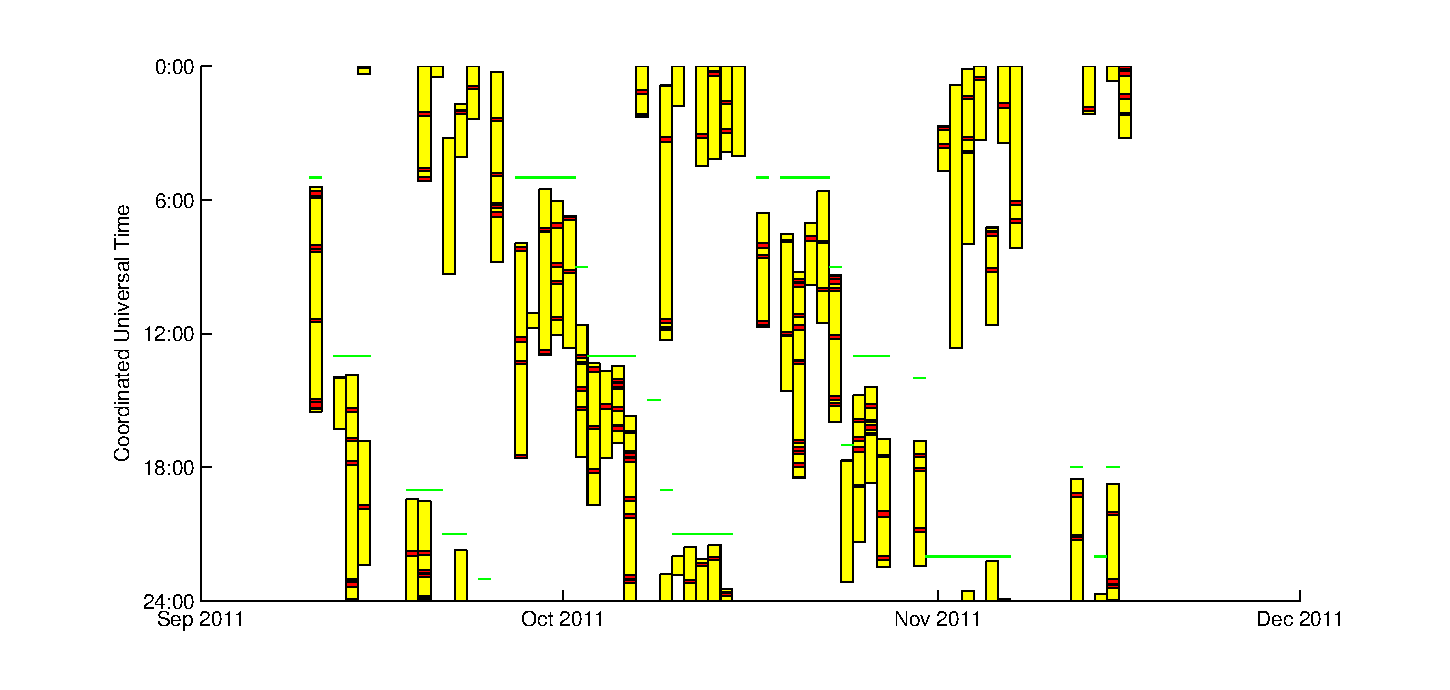
\includegraphics[scale=0.6]{eventTime_sim_example.eps}
  \caption{Example of using patch\_timeCycle\_data.m, plot\_time\_date.m, and plot\_time\_data\_lines.m functions.}
  \label{time_plot}
\end{figure}

\subsection{set\_for\_time\_graph.m}
This function sets limits, ticks, and label of the clock time plot against date. I recommend you to use this function after using above three functions to avoid the hustle of setting the figure. 

\chapter{Functions in ExperimentalTimeData/Code/TimeAnalysisFunction/}
\subsection{calc\_events\_per\_time\_cycle.m}
This function gets an array of times and a two-column array (size a$\times$2) of time cycles, [time1, time2], and return an one-column array of number of runs within each time cycle (size a$\times$1) and a two-column array (size a$\times$2) of the earliest time and the latest time in each time cycles. Following is the example.

\begin{verbatim}
>> time = [0,1,7,8,9,11,13,15];
>> fixedCycle = [0,8.5;13,14];
>> [count,timeCycle] = calc_events_per_time_cycle(time,fixedCycle)

count =

     4
     1


timeCycle =

     0     8
    13    13
\end{verbatim}

%From here!!

\subsection{st2utc\_ch.m}
This function gets Geneva time (UTC+2 or +1) and return UTC (Coordinated Universal Time) considering daylight saving in MATLAB date number.




\chapter{Data Set Classes in ExperimentalTimeData/Class/}
Following functions are for getting data stored at ExperimentalTimeData/DataSets/ folder. 

\section{attempted\_run()}
\label{sec:attempted}
This function gets data of runs that attempted to trap $\bar{H}$. See Section \ref{sec:genAttempted} for details of data you can get. Following is the example of getting data.

\begin{verbatim}
attempted = attempted_run();
run = attempted.run();
spillLog = attempted.spillLogID();
startTime = attempted.startTime();
endTime = attempted.endTime();
run_quench = attempted.run_quench();
dataLog_quench = attempted.dataLogID_quench();




\end{verbatim}

\section{successful\_run()}
\label{sec:successful}


This function provides you all necessary event time data that has been already calculated. It contains five nested functions, 'run', 'utc', 'utc\_jd', 'local', 'type'. Three data inputs are required; year of the data, data with Bias-Right or Bias-Left configuration, and data with accurate or rough event time. Since it calls data from 'EventTimeData.mat' file, the file should be located.This is the example code for running this function.\\
\begin{verbatim}
>> t = event_time();
>> run2010R = t.run('2010','R',0); %get run numbers of 2010 Bias-Right data
>> localTime2010R = t.local('2010','R',0); % get event times in Geneva time
\end{verbatim}

\noindent
Input : (year, RorL, mode)\\
\begin{tabular}{lcl}
year & - & '2011', '2010' or 'all' (string). '2011' for 2011 year's data, '2010' for 2010 year's \\
& & data, 'all' for both\\
RorL & - & 'R', 'L', or 'all'. 'R' for Bias-Right data, 'L' for Bias-Left data, 'all' for both\\
mode & - & 0 for rough event time data ( accurate to a few seconds)\\
\end{tabular}
Output : \\
\begin{tabular}{lcl}
event\_time/run & - & run numbers\\
event\_time/utc & - &   event times in UTC (serial date number)\\
event\_time/utc\_jd & - & event times in UTC (Julian Date)\\
event\_time/local & - &  event times in Geneva time (serial date number)\\
event\_time/type & - & 1 if the event time is calculated by function 'get\_event\_time\_via\_mcp.m' \\
& & 2 if calculated by 'get\_event\_time\_via\_csi.m'\\
& & 0 if calculated by 'get\_entry\_time.m'\\
\end{tabular}\\
Required data : EventTimeData.mat\\

\section{shift\_cycle()}
\label{sec:shift}

\section{spillLog()}
\label{sec:spillLog}




\chapter{Data Directories in ExperimentalTimeData/DataSets}
\section{AttemptedRunData.mat, ShiftTimeData.mat, spillLogData.mat, EventTimeData.mat}
These data are created using functions stored at ExperimentalTimeData/Code/
\section{eventTime\_experiment}
\section{RawData}




\chapter{Miscellaneous}
This chapter is intended to be a place for information that doesn't quite fit anywhere else.

\section{SimulationData/TracerOutput/}
This folder contains the end results of the $\bar{H}$ tracer simulations and this data is used to generate all the simulated data sets.  The data is stored in two different ways: .mat and .ellip files.  The .ellip files are text files and the .mat files are Matlab binary files that are smaller and can be read/written faster than the .ellip files.  Therefore, only use the .ellip files for visual inspection with a text editor.

Each .ellip file in this folder has two columns.  The first  column is the wait time it took (in seconds) for the $\bar{H}$ to hit the trap walls after the quench.  Note that this is \textit{not} the wall time of the event.  The second column is the $z$-position (in meters) of the annihilation with respect to the trap center.  This set of data includes effects from detector smearing and cuts\footnote{Cuts are criteria used to distinguish $\bar{H}$ annihilations from other events, such as those due to cosmic rays.}.  This data is read in automatically by instances of the Position\_Generator class when generating Raw\_Data\_Set instances.

Currently three tracer data sets are included in this directory: MediumSimData, LargeSimData, and AllSimData.  MediumSimData and LargeSimData contain a portion of the full set of simulation output AllSimData, which is ${\sim}$400MB so it is not included in the Dropbox folder.  Each of these has two versions: one in which the rows are randomly oriented (whatever order that they came out of the tracer simulations) and one in which they are sorted by $z$-position.  The sorted versions are used in case a future version of the Position\_Generator class does some interpolation between these event positions.


\end{document}